\chapter{PEOPLE: Predetermined Order, Prunded Label}\label{chapter:peopel}

Das erstellen von Abkürzungen während der Kontraktion eines Knotes $v$ erfordert mindestens $\abs{\text{Vorgänger}} \cdot \abs{\text{Nachfolger}}$ viele Vergleiche, ob eine Kante einzufügen ist.
Wird eine Warteschlange mit Kanten-Differenz benutzt, so sind alleine für die Initalsierung deren Initialsierung $\sum_{v \in V} \abs{\text{Vorgänger}(v)} \cdot \abs{\text{Nachfolger}(v)}$ Vergleiche notwendig.
Für Graphen, welche Knoten mit einem hohem Grad enthalten, kann dies dazu führen, dass die Kontraktion des Graphens nicht in einem sinvollen Zeitrahmen berechenbar ist.
Trotzdem wäre es praktisch, wenn sich die Query-Zeiten von Contraction Hierarchirs und Hierachical Hub Labeling auch auf sie übertragen ließen.

Um die Nachfolgende Definition vorzubereiten, betrachten wir ein Beispiel.
Sei $G = (V, E)$ mit $V \supset \{ u, v, w \}$ und $E = \{ (u, v, {spd}((u, v))), (v, w, {spd}((v, w))) \}$, ein Produkt einer Kontraktion, also zu Beginn mehr Kanten und nicht-isolierte Knoten entiehlt
Es soll nun $v$ kontraktiert werden.
Hierfür wir eine Kante $(u, w, {spd}((u, w)))$ eingefügt und die Kanten $(u, v), (v, w)$ entfernt.
Was bedeuted dies für den enstehenden Contracted Graph $C$?
\begin{enumerate}
    \item
          Alle Knoten, einschließlich $v$ haben ein niedriges Level als $u$ und $w$.
          Inbesondere haben alle Knoten auf allen kürzesten Pfaden von $u$ nach $w$, also die, die bereits kontraktiert wurden, ein niedrigeres Level.

    \item
          $(u, w) \in E_u$ gilt genau dann, wenn $w$ das größte Level auf allen Pfaden von $u$ nach $w$.
          $(w, u) \in E_d$ gilt, wenn $u$ das größte Level hat.
\end{enumerate}

Es kann nun gezeigt werden, dass auch die Rückrichtung gilt, also dass basienden auf dieser Chracterisierung ein Contracted Graph gebildet werden kann.

\begin{definition}[Upward Graph]\label{people:def:upward_graph}
    Sei $G = (V, E)$ und ${vtl}$ eine \emph{vertex-to-level} Funktion dazu. Dann ist $G_u = (V, E_u)$ ein \emph{upward Graph} zu $G$ wenn für jeden Knoten $t \in V$ gilt:

    \begin{itemize}
        \item
              $E_u$ enthält nur Kanten $(t, h, d)$, $h \in V$ und $d \in \mathbb{R}^+$ mit ${vtl}$, für die es einen $t-h$ Pfad der Länge $d$ gibt, so dass auf ihm $h$ das größte und $t$ das zweitgrößte enthält.

        \item
              $E_u$ enthält alle Kante $(t, h, {spd}((t, h)))$ mit $h \in V$, für die allen $t-h$ Pfaden $h$ das größte und $t$ zweitgröste Level hat
    \end{itemize}
\end{definition}

Betrachten wir das ganze an dem bereits definierten Beispielgraph.
Sei ${vtl}$ definiert durch die Abbildung in \autoref{ch::fig::vtl_abbildung} definiert.
Durch Anwendung der Definition \ref{people:def:upward_graph} ergibt sich der in \autoref{ch::fig::upward_graph} gezeigte Upward Graph.

\begin{table}[ht]
    \centering
    \begin{tabular}{lllllllllllll}
        Vertex & a & b & c & d & e & f & g & h & i & j  & k & \\
        Level  & 8 & 7 & 3 & 6 & 2 & 5 & 1 & 4 & 0 & 10 & 9 &
    \end{tabular}
    \caption{${vtl}$ Beispielfunktion}
    \label{ch::fig::vtl_abbildung}
\end{table}


\begin{figure}[ht]
    \centering
    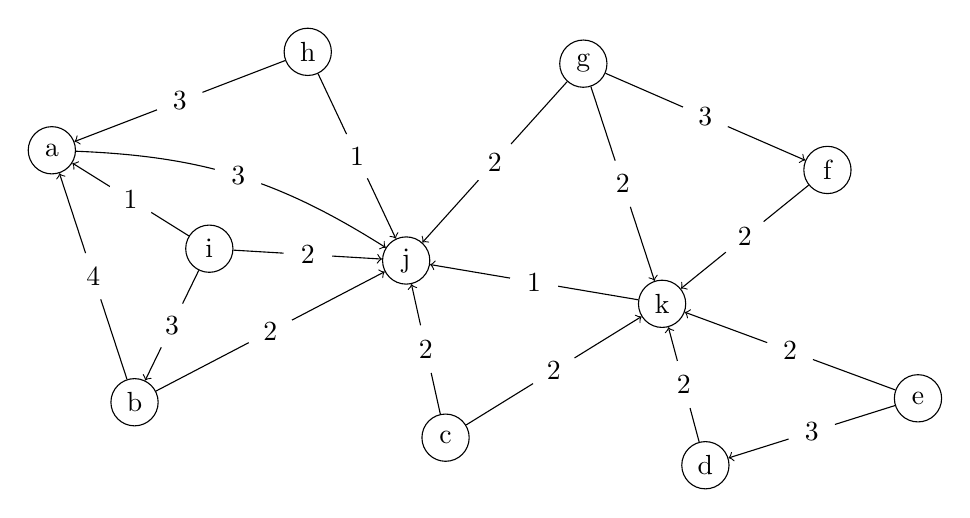
\begin{tikzpicture}
        % Nodes
        \node[circle, draw, minimum size=0.6cm, inner sep=0pt] at (0.5* 0.0, 0.5* 8.5)  (a)    {a};
        \node[circle, draw, minimum size=0.6cm, inner sep=0pt] at (0.5* 2.1, 0.5* 2.1)  (b)    {b};
        \node[circle, draw, minimum size=0.6cm, inner sep=0pt] at (0.5* 10.0, 0.5* 1.2)  (c)    {c};
        \node[circle, draw, minimum size=0.6cm, inner sep=0pt] at (0.5* 16.6, 0.5* 0.5)  (d)    {d};
        \node[circle, draw, minimum size=0.6cm, inner sep=0pt] at (0.5* 22.0, 0.5* 2.2)  (e)    {e};
        \node[circle, draw, minimum size=0.6cm, inner sep=0pt] at (0.5* 19.7, 0.5* 8.0)  (f)    {f};
        \node[circle, draw, minimum size=0.6cm, inner sep=0pt] at (0.5* 13.5, 0.5* 10.7)  (g)    {g};
        \node[circle, draw, minimum size=0.6cm, inner sep=0pt] at (0.5* 6.5, 0.5* 11.0)  (h)    {h};
        \node[circle, draw, minimum size=0.6cm, inner sep=0pt] at (0.5* 4.0, 0.5* 6.0)  (i)    {i};
        \node[circle, draw, minimum size=0.6cm, inner sep=0pt] at (0.5* 9.0, 0.5* 5.7)  (j)    {j};
        \node[circle, draw, minimum size=0.6cm, inner sep=0pt] at (0.5* 15.5, 0.5* 4.6)  (k)    {k};


        \draw[->]  (a) edge[bend left=15] node[circle, fill=white] {3} (j);

        \draw[->]  (b) edge node[circle, fill=white] {4} (a);
        \draw[->]  (b) edge node[circle, fill=white] {2} (j);

        \draw[->]  (c) edge node[circle, fill=white] {2} (j);
        \draw[->]  (c) edge node[circle, fill=white] {2} (k);

        \draw[->]  (d) edge node[circle, fill=white] {2} (k);

        \draw[->]  (e) edge node[circle, fill=white] {3} (d);
        \draw[->]  (e) edge node[circle, fill=white] {2} (k);

        \draw[->]  (f) edge node[circle, fill=white] {2} (k);

        \draw[->]  (g) edge node[circle, fill=white] {3} (f);
        \draw[->]  (g) edge node[circle, fill=white] {2} (j);
        \draw[->]  (g) edge node[circle, fill=white] {2} (k);

        \draw[->]  (h) edge node[circle, fill=white] {3} (a);
        \draw[->]  (h) edge node[circle, fill=white] {1} (j);

        \draw[->]  (i) edge node[circle, fill=white] {1} (a);
        \draw[->]  (i) edge node[circle, fill=white] {3} (b);
        \draw[->]  (i) edge node[circle, fill=white] {2} (j);


        \draw[->]  (k) edge node[circle, fill=white] {1} (j);
    \end{tikzpicture}
    \caption{Upward Graph des Beispielgraphs}
    \label{ch::fig::upward_graph}
\end{figure}

Die Definition des Downward Graphens erfolgt nun analog zu der des Upward Graphens:

\begin{definition}[Downward Graph]
    Sei $G = (V, E)$ und ${vtl}$ eine \emph{vertex-to-level} Funktion dazu. Dann ist ein upward Graph des Umkehrgraphens $G^T$ ein \emph{downward Graph} zu $G$.
\end{definition}

Wenn ein Graph ungerichtet ist, dann ist er äuivalent zu seinem Umkehrgraphen und dann ist auch der Upward und Downward Graph äuivalent.
Daher entspricht \autoref{ch::fig::upward_graph} gleichzeitig auch dem Downward Graph des Beispielgraphens.

\todo{Beweis Korrektheit}

\section{Contracted Graph Algorithmus}

Das Berechnen aller kürzesten Pfade zwischen zwei Knoten ist aufwändig, daher wird zum Berechnen eines so defineirten Contracted Graphens ein ähnlichen Trick angewendet, wie er bei der Knoten Kontraktion angewandt wird:
Wir fügen Kanten ein, sobald wir \emph{einen} optimalten $t-h$ Pfad gefunden haben, auf dem $h$ das größte und $t$ das zweitgrößte Level hat.
Dies ist hinreichend um die Bedingung zu erfüllen, fügt im Zweifel jedoch mehr Kanten als notwendig ein.

Um einen Upward Graphen zu berechnen, wird für jeden Knoten $t \in V$ eine angepasste Dijkstra Suche ausgeführt, bei der für jeden Knoten jeweils notiert wird, was größte Level auf dem Pfad zur Wurzel ist.
Dies Information kann mit der \emph{max-on-path} Funktion ${mop}$ abegrufen werden.
Ein Knoten $h \in V$, $h \neq t$ ist der Kopf eine Upward Graph Kante, für die gilt, dass ${mop}(h) = {vtl}(h)$ und ${mop}({pre}(h)) = {vtl}(t)$.
Das Gewicht der Kante kann der Dijkstra Suche entommen werden.
Die Suche kann abgebrochen werden, wenn nur noch Knoten für alle nicht-expandierten Knoten $h$ ${mop}({pre}(h)) > {vtl}(h)$ gilt.
Betrachten wir dies am Knoten $a$ im Beispielgraphen:

\begin{figure}[ht]
    \centering
    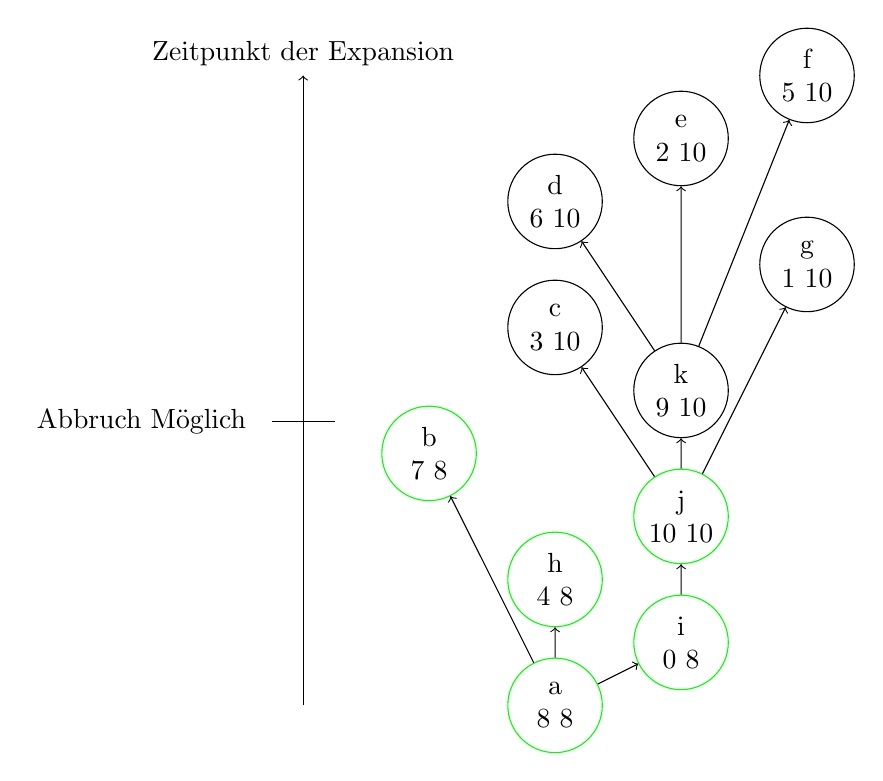
\begin{tikzpicture}[scale=0.8]
        % Nodes
        % a & b & c & d & e & f & g & h & i & j & k & 
        % 8 & 7 & 3 & 6 & 2 & 5 & 1 & 4 & 0 & 10 & 9 & 

        \node[circle, draw=green, minimum size=1.2cm, inner sep=0pt , align=center] at (2* 1, 0)  (a)    {a\\8 8};
        \node[circle, draw=green, minimum size=1.2cm, inner sep=0pt , align=center] at (2* 0, 4)  (b)    {b\\7 8};
        \node[circle, draw, minimum size=1.2cm, inner sep=0pt , align=center] at (2* 1, 6)  (c)    {c\\3 10};
        \node[circle, draw, minimum size=1.2cm, inner sep=0pt , align=center] at (2* 1, 8)  (d)    {d\\6 10};
        \node[circle, draw, minimum size=1.2cm, inner sep=0pt , align=center] at (2* 2, 9)  (e)    {e\\2 10};
        \node[circle, draw, minimum size=1.2cm, inner sep=0pt , align=center] at (2* 3, 10)  (f)    {f\\5 10};
        \node[circle, draw, minimum size=1.2cm, inner sep=0pt , align=center] at (2* 3, 7)  (g)    {g\\1 10};
        \node[circle, draw=green, minimum size=1.2cm, inner sep=0pt , align=center] at (2* 1, 2)  (h)    {h\\4 8};
        \node[circle, draw=green, minimum size=1.2cm, inner sep=0pt , align=center] at (2* 2, 1)  (i)    {i\\0 8};
        \node[circle, draw=green, minimum size=1.2cm, inner sep=0pt , align=center] at (2* 2, 3)  (j)    {j\\10 10};
        \node[circle, draw, minimum size=1.2cm, inner sep=0pt , align=center] at (2* 2, 5)  (k)    {k\\9 10};


        \draw[->]  (a) edge (b);
        \draw[->]  (a) edge (h);
        \draw[->]  (a) edge (i);
        \draw[->]  (j) edge (c);
        \draw[->]  (i) edge (j);
        \draw[->]  (k) edge (d);
        \draw[->]  (j) edge (k);
        \draw[->]  (k) edge (e);
        \draw[->]  (k) edge (f);
        \draw[->]  (j) edge (g);

        \draw[->] (-2, 0) -- (-2, 10) node[above] {Zeitpunkt der Expansion};

        \draw (-2.5, 4.5) -- (-1.5, 4.5) node[left=1cm] {Abbruch Möglich};

    \end{tikzpicture}
    \caption{Brute-Force Suche}
    \label{ch:fig:brute_force_suchbaum}
\end{figure}

Die Informtion des größten Levels auf dem Pfad zur Wurzel kann dabei beim Update eines Kontens übertragen werden, indem das Maximum des bisherigen größten Levels und das Level des upgedateten Knoten gebildet wird.
Die Abbruchbedingung kann durch die Verfolgung einer Menge an \emph{lebendigen} erzielt werden, sobald diese keine Knoten mehr entählt, kann die Suche abgebrochen werden.
Zu beginn ist nur der Startknoten lebendig, die Lebendigkeit wird jeweils an die Kinder vererbt.
Ein Knoten stirbt, nachdem er expandiert wurde oder wenn er den Kopf einer Kante bildet.
Gibt es keine lebendigen Knoten mehr, so kann die Suche abgebrochen werden.
In dem verwendeten Beispiel wäre dies etwa nach der Expansion von $b$ der Fall.
Die Berechung ist \emph{embarrassingly parallel}, da jeder Knoten für sich selbst Berechnet werden kann.
Der textuell beschriebene Algorithmus wird dann wie folgt formal definiert:

\begin{algorithm}[ht]
    \caption{Contracted Graph Brute Force Suchalgorithmus}
    \begin{algorithmic}[1]
        \Require Graph $G = (V, E)$, vertex-to-level Funktion ${vtl}$, Startknoten $s \in V$, Zielknoten $t \in V$
        \Ensure $E_s$
        \State // Initialisiere Distanz- und Vorgänger-Funktion
        \ForAll{$v \in V$}
        \State ${dist}(v) \leftarrow \infty$
        \State ${pre}(v) \leftarrow {none}$
        \EndFor


        \State
        \State // Initialisiere Suche
        \State ${dist}(s) \leftarrow 0$
        \State $Q\leftarrow \{ s \}$
        \State ${pre}(s) \leftarrow s$

        \State
        \State // Initialisiere max-on-path
        \State ${mop}(s) \leftarrow {vtl}(s)$
        \State $E_s \leftarrow \{ \}$
        \State ${alive} \leftarrow \{ s \}$

        \State
        \While{$Q \neq \emptyset \land {alive} \neq \emptyset$}
        \State $u \leftarrow{extract\_min}(Q)$\label{graphs:dijkstra:pop}

        \State
        \State // Beende frühzeitig wenn Zielknoten gefunden wurde
        \If {$u \neq s \land {mop}(u) = {vtl}(u)$}
        \State $E_s \leftarrow E_s \cup \{ (s, u, {dist}(u)) \}$
        \State ${alive} \leftarrow {alive} \setminus \{ s \}$
        \EndIf

        \State
        \State // Aktualisiere Nachbarn
        \ForAll{$(u, v, w) \in E$}
        \If {${dist}(u) + w < {dist}(v)$}
        \State ${dist}(v) \leftarrow {dist}(u) + w$
        \State ${pre}(u) \leftarrow v$
        \State $Q = Q \cup \{ v \}$
        \State
        \State // setze max\_level\_path
        \State ${mop}(v) \leftarrow \max({mop}(v), {vtl}(v))$
        \If {$u \in {alive}$}
        \State ${alive} \leftarrow {alive} \cup \{ s \}$
        \EndIf
        \EndIf
        \EndFor


        \State ${alive} \leftarrow {alive} \setminus \{ s \}$

        \EndWhile

        \State
        \State \Return $E_s$
    \end{algorithmic}
\end{algorithm}

\subsection{Abkürzung Problem}

Es liegt nahe als abgekürzten Knoten den Knoten mit dem dritthöchsten Level auszuwählen und sich darauf zu verlassen, dass die Suche von diesem Knoten aus die nächsen Abkürzung findet, und so weiter.
Dies wäre praktisch, da dann jeder Shortcut nur einmal erstellt werden müsste.
Zwei Gründe können jedoch dagegen sprechen:
Wird als Graph eine Datenstruktur verwendet, welche die Nachbarn nicht in einer definierten Ordnung ausgibt (etwa ein Hashset), können zwei Suchen von bzw. zu einem Knoten zwei Unterschiedliche kürzeste Pfad Bäume bilden.
Eine nicht stabile Prioritätswarteschlange kann ebenfalls den gleichen Effekt herbeiführen.

\autoref{ch:fig:problem_shortcut} zeigt eine Situation, in der so ein Problem auftreten kann.
Für den Knoten $a$ wird die Kante $(a, e)$ mit dem abekürztem Knoten $d$ gefunden.
Wir verlassen uns darauf, dass die Suche von $d$ aus die Abkürzung $(d, a)$ mit dem Knotem $b$ findet.

Die Lösung hierfür ist, dass die Abkürzungen, welche benötigt werden, um die ursprüngliche Abkürzung vollständiz zu entpacken, ebenfalls erstellt werden.
Diese werden aber mit einer hohen Wahrscheinlichkeit von den Bruteforcing der jeweils abgekürzten Knoten endeckt.
Der Speichermehrbedarf hierbei kann ein Problem für die Umsetzbarkeit des Algorithmus werden, weshalb ein Mechanismus verwendet werden sollte, welcher die mehrfache Speicherung verhindet, etwa eine HashMap.
Dies führt allerdings zu einem Performance-Hit, da dies synchroniesert werden muss.
Für denn Fall, dass nur die kürzesten Pfad Abstände Interesannt sind, kann und sollte hierauf verzichtet werden.

\begin{figure}[ht]
    \centering

    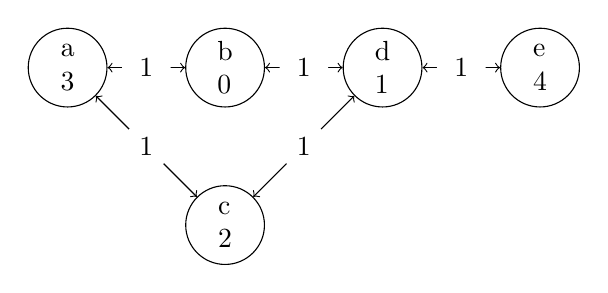
\begin{tikzpicture}
        % Nodes
        \node[circle, draw, minimum size=1cm, inner sep=0pt, align=left] at (2*0, 2*0)  (a)    {a\\3};
        \node[circle, draw, minimum size=1cm, inner sep=0pt, align=left] at (2*1, 2*0)  (b)    {b\\0};
        \node[circle, draw, minimum size=1cm, inner sep=0pt, align=left] at (2*1, 2*-1)  (c)    {c\\2};
        \node[circle, draw, minimum size=1cm, inner sep=0pt, align=left] at (2*2, 2*0)  (d)    {d\\1};
        \node[circle, draw, minimum size=1cm, inner sep=0pt, align=left] at (2*3, 2*0)  (e)    {e\\4};


        \draw[<->]  (a) edge node[circle, fill=white] {1} (b);
        \draw[<->]  (b) edge node[circle, fill=white] {1} (d);
        \draw[<->]  (d) edge node[circle, fill=white] {1} (e);


        \draw[<->]  (a) edge node[circle, fill=white] {1} (c);
        \draw[<->]  (c) edge node[circle, fill=white] {1} (d);
    \end{tikzpicture}
    \caption{Problem beim Shortcut erstellen}
    \label{ch:fig:problem_shortcut}
\end{figure}

\section{Hub Labels Algorithmus}

Der gleiche Idee zur Erstellung eins Contracted Graphens lässt sich auch auf die Erstellung eines Hub Graphens anwenden.
Hierfür wird die Abbruchbedingung durch die Lebendigkeit entfernt.

Der Aglorithmus kann auch dafür benutzt werden, die Qualität (durschnitliche Label Size) einer vertex-to-level Funktion anzugeben, ohne den kompletten Hub Graphen zu berechnen.
Hierfür würd für $n$ Knoten das Label berechnet und die größte des Labels angegeben.
Das ist vielleicht interesannt, um gute Top-Down Orderings zu finden (unter der Annahme, dass dieser Orderings auch effizientes Kontraktieren zulassen).
Da sich das recht schnell berechnen lässt kann man vielleicht einen Solver dafür einsetzen?

Analog dazu kann für einen Knoten $v$ auch der CH Suchbaum berechnet werden, indem iterative für jeden gefunden Knoten wieder die CH Kanten berechnet werden. Das ist potentiell aber etwas teurer.